% Shared manuscript content for both bioRxiv and Oxford Bioinformatics versions
% This file contains only the main text content
% Metadata (title, authors, abstract, etc.) is defined in the main template files

\section{Introduction}
Reconstructing viral genomes from metagenomic sequencing data presents considerable computational challenges, particularly for viruses exhibiting extensive genetic diversity \citep{Baaijens2017-hw,Meleshko2021-gb}. This diversity is further compounded by segmented genomes in families like influenza, rotavirus, and bunyaviruses, where individual segments can evolve under distinct selective pressures and reassort, contributing to a complex landscape for genome reconstruction. While pipelines are often designed to target specific viruses and their subtypes \citep{Shepard2016-uh}, accurate and complete genome reconstruction of samples with unknown references typically requires manual curation of contigs and reference matching \citep{de_Vries2021-po}. This manual curation process is time-consuming, making it impractical for large-scale metagenome studies or rapid response scenarios that involve emerging viral outbreaks of unknown origin.

To address these limitations, we developed \href{https://github.com/nf-core/viralmetagenome}{nf-core/ viralmetagenome}, a comprehensive pipeline specifically designed for untargeted viral genome reconstruction. The pipeline is developed using Nextflow \citep{Di-Tommaso2017-nz} within the nf-core framework \citep{Ewels2020-kk}, ensuring reproducibility through containerization with Docker \citep{Merkel2014-hn} and Singularity \citep{Kurtzer2017-iw}, and enabling portability across computational platforms such as local desktops, high-performance clusters and cloud environments.

\section{Pipeline Description}

\href{https://github.com/nf-core/viralmetagenome}{nf-core/viralmetagenome} implements an automated workflow performing \textit{de novo} assembly, reference matching, and iterative consensus refinement for the reconstruction of  viral genomes without prior target knowledge. The pipeline consists of five major stages: read preprocessing, metagenomic diversity assessment, contig assembly and scaffolding, iterative consensus refinement with variant analysis, and quality control (Figure~\ref{fig:pipeline-workflow}). While this manuscript highlights key differences between particular tools, unless otherwise specified, the pipeline offers multiple options to accommodate established user workflows and preferences. In depth tool details are available in Supplementary Table 1.

\begin{figure*}[htbp]
    \centering
    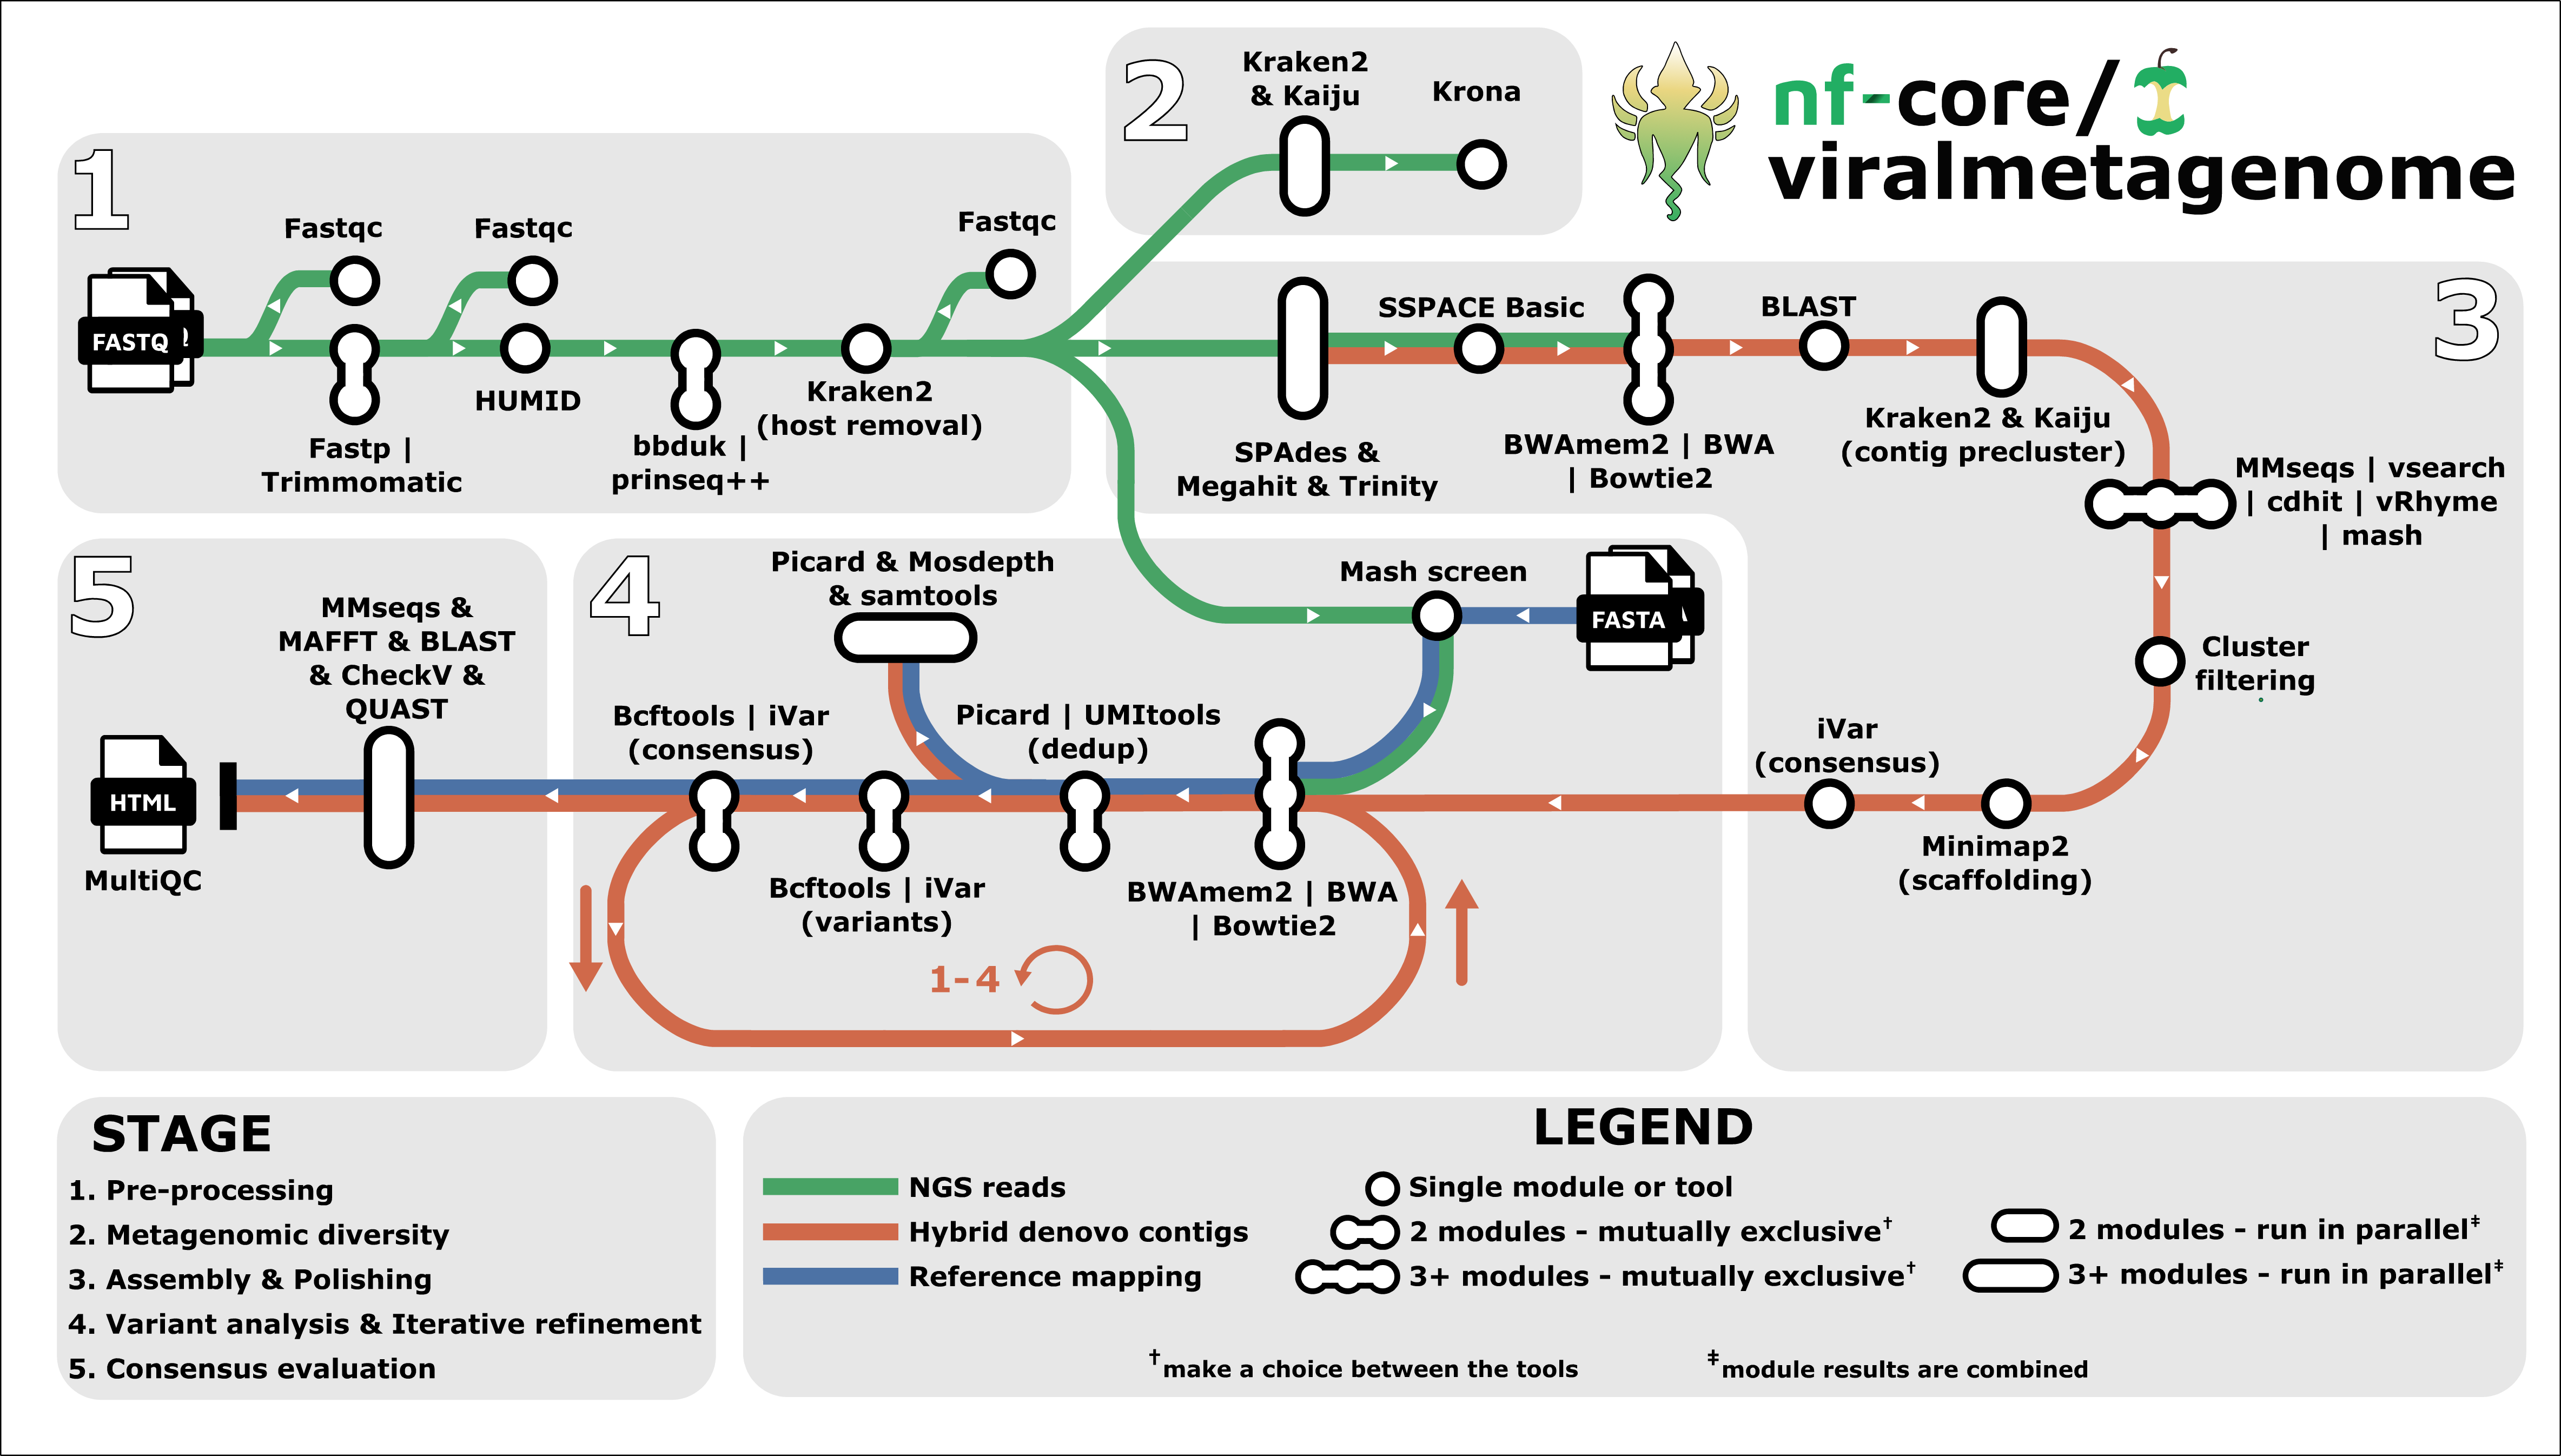
\includegraphics[width=1\textwidth]{Fig/fig1.png}
    \caption{Visual overview of the nf-core/viralmetagenome pipeline for untargeted viral genome reconstruction. \href{https://github.com/nf-core/viralmetagenome}{nf-core/viralmetagenome} processes short-read data through pre-processing, metagenomic diversity assessment, \textit{de novo} assembly with multiple assemblers, scaffolding with automated reference identification and contig taxonomy-guided clustering, and iterative consensus refinement through read mapping and variant calling. Quality control metrics, assembly statistics, and coverage data are integrated into interactive MultiQC reports and standardised overview tables for downstream analysis.}
    \label{fig:pipeline-workflow}
\end{figure*}

\subsection{Read preprocessing}

Input reads provided via sample sheets containing sample names and short-read FASTQ paths are preprocessed using FastQC and have their adapters trimmed with fastp \citep{Chen2018-tu} (default) or Trimmomatic \citep{Bolger2014-si}. Fastp is overall faster and has automated adapter detection and trimming \citep{Chen2018-tu}. UMI deduplication is implemented using HUMID \citep{LarosUnknown-nx} and once reads are mapped to a reference with UMI-tools \citep{Smith2017-nk}. Multiple sequencing runs are merged after trimming by specifying merge group identifiers in the sample sheet. Complexity filtering with bbduk \citep{BushnellUnknown-qy} or PRINSEQ++ \citep{Cantu2019-vs} removes low-complexity sequences containing repetitive elements where host reads are removed with Kraken2 \citep{Wood2019-jl}.

\subsection{Metagenomic diversity assessment}

Taxonomic classification of preprocessed reads is performed using two complementary approaches - Kaiju \citep{Menzel2016-tz} and Kraken2 \citep{Wood2019-jl} - to maximise detection sensitivity across diverse viral families. Results from both classifiers are visualised using Krona \citep{Ondov2011-yp}.

\subsection{{\it De novo} assembly and clustering}

The assembly workflow implements multi-assembler approaches followed by clustering and scaffolding. \textit{De novo} assembly is performed using SPAdes \citep{Meleshko2021-gb} (RNAviral mode), MEGAHIT \citep{Li2016-sd}, and Trinity \citep{Grabherr2011-ef}, capitalizing on distinct algorithmic strengths to maximise genome recovery across diverse viral families and variable read depths.

Reference identification uses BLASTn \citep{Altschul1990-sy} against the Reference Viral Database (RVDB) \citep{Goodacre2018-dw}, retaining top five hits to facilitate identification of related genomic segments and appropriate reference sequences for contig scaffolding and clustering.

Clustering is performed in two sequential stages. First, taxonomic pre-clustering groups contigs based on taxonomic classification using Kraken2 \citep{Wood2019-jl} and Kaiju \citep{Menzel2016-tz}, with optional filtering to focus on specific taxonomic clades for more targeted analyses. Second, nucleotide similarity clustering within taxonomic groups is performed using CD-HIT-EST \citep{Li2006-nj}, VSEARCH \citep{Rognes2016-ju}, MMseqs2 \citep{Steinegger2017-ci}, vRhyme \citep{Kieft2022-km}, or Mash \citep{Ondov2019-bo}. All tools are valid options, though performance may vary depending on the dataset \citep{Zielezinski2025-vl,Steinegger2017-ci}.

As an optional filtering step of contig clusters, after assembly and extension, reads can be mapped to all contigs using BWA-MEM2 \citep{Vasimuddin2019-rb} (default), BWA \citep{Li2013-pp}, or bowtie2 \citep{Langmead2019-wx}. Clusters are filtered based on the total percentage of reads mapping to all contigs within a cluster, allowing identification and removal of clusters that likely represent assembly artefacts resulting from low read coverage.

For the final scaffolding step, all cluster members are mapped to the cluster representative or centroid using Minimap2 \citep{Li2018-gi}, followed by consensus calling with iVar \citep{Grubaugh2019-xd} to generate reference-assisted assemblies. Regions with zero coverage depth can optionally be represented by the reference genome to produce a more complete scaffold genome for consensus calling.

\subsection{Iterative consensus refinement and variant calling}

The consensus module supports external reference-based analysis and scaffold refinement. Users can provide a separate reference genome or reference set for each sample with \texttt{--mapping\_constraints}; when a reference set is provided, the most similar can be selected using Mash \citep{Ondov2019-bo}.

Scaffold refinement performs up to 4 iterative cycles (default 2). Each iteration maps reads using BWA-MEM2 \citep{Vasimuddin2019-rb}, BWA \citep{Li2013-pp}, or bowtie2 \citep{Langmead2019-wx} to the consensus, followed by variant calling with BCFtools \citep{Danecek2021-je} or iVar \citep{Grubaugh2019-xd}. Benchmarking by Bassano et al. \citep{Bassano2022-cl} showed that BCFtools outperformed iVar in precision and recall, where iVar identified more low frequency variants. Users are recommended to consider prioritising sensitivity or specificity when selecting the variant caller.

\subsection{Consensus Quality Control}

Quality control employs CheckV \citep{Nayfach2021-wl} for completeness estimates, BLASTn \citep{Altschul1990-sy} for reference similarity, and MMseqs2 \citep{Steinegger2017-ci} against the annotated database Virosaurus \citep{Gleizes2020-rq}. These analyses enable species identification, genomic segment classification, host prediction, and any other additional metadata embedded within the reference databases.

The refinement progression is evaluated through sequence alignment with MAFFT \citep{Katoh2002-ox}, which compares final consensus genomes against \textit{de novo} contigs, intermediate consensus sequences from iterative cycles, and the scaffolding reference. All tool metrics are compiled into an interactive MultiQC report \citep{Ewels2016-hs}. Additionally, key metrics are extracted from the MultiQC report and compiled into standalone overview tables to facilitate downstream analysis across all processed samples.

\section{Applications}

To assess the performance of nf-core/viralmetagenome under challenging scenarios, we simulated coinfection scenarios by mixing paired-end reads from public HIV-1 genomes with varying diversity (80-99\%), resulting in 13 samples (See supplementary table 2). Nf-core/viralmetagenome successfully identified coinfections in all mixed samples when genetic similarity was low to moderate ($\leq$ 96.7\%).

We validated nf-core/viralmetagenome performance on real metagenomic samples spanning human and plant pathogens. Here, the pipeline successfully generated high-quality or near-complete genomes across viral families including segmented (Lassa virus, Orthonairovirus, Tomato spotted wilt tospovirus) and non-segmented viruses (SARS-CoV-2, West Nile virus, Potato virus Y, Youcai mosaic virus, and Monkeypox virus).

Processing 28 samples (supplementary methods) required 412 CPU hours and a maximum of 79GB RAM on an HPC, excluding taxonomic classification steps. The automated reference selection offers substantial improvements over manual curation by reducing processing time while preserving reconstruction accuracy. Performance correlates strongly with reference database comprehensiveness, as consensus genomes tended to be more complete and similar to the true consensus sequence when the scaffolding reference was closer to the true viral genome. This emphasizes the need to keep databases like RVDB \citep{Goodacre2018-dw} and Virosaurus \citep{Gleizes2020-rq} up-to-date. Since nf-core/viralmetagenome is primarily designed for eukaryotic viruses, bacteriophage analysis requires different approaches and users are encouraged to explore pipelines targeting phages such as VIRify \citep{Rangel-Pineros2022-wv}, VIBRANT \citep{Kieft2020-aq}, VirSorter2 \citep{Guo2021-rf}.


\section{Conclusion}

nf-core/viralmetagenome addresses a critical need in viral genomics by providing an automated, scalable solution for untargeted viral genome reconstruction. The pipeline successfully automates the traditionally time-consuming and manual execution process of viral genome assembly from short-read metagenomic data through its integrated workflow of \textit{de novo} contig assembly, automated reference selection, clustering algorithms, and iterative refinement strategies.

Our validation demonstrates the pipeline's broad applicability across diverse eukaryotic viral families, achieving high-quality genome reconstruction while ensuring reproducibility and ease of deployment across different computational environments.

As viral surveillance and outbreak response increasingly rely on metagenomic sequencing, automated pipelines like nf-core/viralmetagenome will be essential for the timely identification of pathogen strains. The pipeline represents a significant step forward in making viral genome reconstruction accessible to researchers without requiring extensive bioinformatics expertise, facilitating broader adoption of metagenomic approaches in viral research and public health applications.


\section*{Acknowledgments}
 J.K, P.L. and L.E.K  acknowledge support from the Research Foundation - Flanders (Fonds voor Wetenschappelijk Onderzoek – Vlaanderen, G005323N and G051322N, 1SH2V24N, 12X9222N).

\section*{Author Contributions}
J.K. designed and implemented the pipeline, performed validation analyses, and wrote the manuscript. P.L. and L.E.K. supervised the project and provided critical feedback. The nf-core community contributed to maintaining the pipeline. All authors reviewed and approved the final manuscript.

\section*{Conflict of Interest}
The authors declare no competing interests.

